\documentclass[tikz,border=10pt]{standalone}
\usetikzlibrary{calc}
\begin{document}
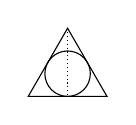
\begin{tikzpicture}
  \coordinate (A) at (1,2);
  \coordinate (B) at ($(A)+(1,0)$);
  \coordinate (C) at ($(A)+(60:1)$);
  \draw (A) -- (B) -- (C) --cycle;
  \draw ($(A)!0.5!(B)+(0,{sqrt(3)/6})$) circle({sqrt(3)/6});
  \draw[densely dotted] (C) -- ($(A)!(C)!(B)$);
\end{tikzpicture}
\end{document}
